\documentclass[11pt,aspectratio=43,ignorenonframetext,t]{beamer}
% Uses fontspec - assumes compiled with LuaLaTeX or similar
% The above \documentclass is for making slides. If making handouts use:
%\documentclass[11pt,a4paper]{article} 
%\usepackage{beamerarticle}
%\setjobnamebeamerversion{main.beamer}

% See https://github.com/CASSON-LAB/uom_beamer_template
% for details on license, further useage information and similar

\graphicspath{fig/aula1/}
%%%%%%%%%%%%%%%%%% DOCUMENT SETUP %%%%%%%%%%%%%%%%%%

% Presentation settings
\mode<presentation>{
  \usetheme[framenumber,titleframestart=1]{UoM_alex}
  \usefonttheme{professionalfonts} % using non standard fonts for beamer
  \usefonttheme{serif}             % set font to Arial
  \usepackage{fontspec}
  \setmainfont[Ligatures=TeX]{Arial}
}

% Handout settings
\mode<article>{
  \usepackage{fullpage}                  % use full page
  \usepackage{fontspec}                  % set font to Arial
    \setmainfont[Ligatures=TeX]{Arial}
  \setlength{\parskip}{1.5\baselineskip} % correct beamer line spacings
  \setlength{\parindent}{0cm}
  \usepackage{enumitem}
    \setlist[itemize]{topsep=0pt}
  \definecolor{uomlinkblue}{HTML}{0071BC}
}


% Packages

\usepackage{listings}
% Configurando layout para mostrar codigos C++
\usepackage{listings}
\lstset{
  language=Java,
  basicstyle=\ttfamily\small, 
  keywordstyle=\color{blue}, 
  stringstyle=\color{orange}, 
  commentstyle=\color{gray}, 
  extendedchars=true, 
  showspaces=false, 
  showstringspaces=false, 
  numbers=left,
  numberstyle=\tiny,
  breaklines=true, 
  backgroundcolor=\color{blue!7},
  breakautoindent=true, 
  captionpos=b,
  xleftmargin=0pt,
}
\usepackage{graphicx}  % for graphics files
  \graphicspath{ {./fig/} }
\usepackage{amsmath}   % assumes amsmath package installed
  \allowdisplaybreaks[1] % allow eqnarrays to break across pages
\usepackage{amssymb}   % assumes amsmath package installed 
\usepackage{hyperref} % add hyperlinks to document. Settings are for accessiblity
  \hypersetup{
    colorlinks=true,
    linkcolor=uomlinkblue,
    filecolor=uomlinkblue,      
    urlcolor=uomlinkblue,
	pdflang={en-GB},
}
\usepackage[document]{ragged2e} % left aligned text for accessibility
% experimental - does fundamentally work, if with quite a bit of effort
%\usepackage{axessibility} % LaTeX readable equations for accessibility
%  \tagpdfsetup{tabsorder=structure,uncompress,activate-all,interwordspace=true}
%  \pdfextension catalog{/Lang (en-GB)}
%  \RequirePackage{luacode}
%  \directlua{require("axessibility.lua")}
\usepackage{unicode-math} % unicode maths for accessibility
\usepackage{pdfcomment} % for alt text for accessibility
\usepackage{rotating}  % allow portrait figures and tables
\usepackage{subfigure} % allow matrices of figures
\usepackage{float}     % allows H option on floats to force here placement
\usepackage{multirow}  % allows merging of rows in tables
\usepackage{tabularx}  % allows fixed width tables
\usepackage{ctable}    % modifies \hline for use in table
\usepackage{bm}        % allow bold fonts in equations
\usepackage{pgf}       % allow graphics manipulation
\usepackage{media9}    % allow interactive flash files to be embedded
  \addmediapath{../media}
\usepackage{etoolbox}
  \makeatletter \preto{\@verbatim}{\topsep=0pt \partopsep=0pt} \makeatother  
  
% Custom commands
\newcommand{\matlab}{\emph{\sc{Matlab}}}
\newcommand{\maple}{\emph{\sc{Maple}}}
\newcommand{\simulink}{\emph{\sc{Simulink}}}
\newcommand{\dc}{d.c.}
\newcommand{\ac}{a.c.}
\newcommand{\rms}{RMS}
\newcommand{\wgn}{{\tt wgn}}
\newcommand{\sus}[1]{$^{\mbox{\scriptsize #1}}$}
\newcommand{\sub}[1]{$_{\mbox{\scriptsize #1}}$}
\newcommand{\chap}[1]{Chapter~\ref{#1}}
\newcommand{\sect}[1]{Section~\ref{#1}}
\newcommand{\fig}[1]{Fig.~\ref{#1}}
\newcommand{\tab}[1]{Table~\ref{#1}}
\newcommand{\equ}[1]{(\ref{#1})}
\newcommand{\appx}[1]{Appendix~\ref{#1}}
\newcommand{\degree}{\ensuremath{^\circ}}
\newcommand{\Vrms}{Vrms}
\newcommand{\Vpp}{V\sub{pp}}
\newcommand{\otoprule}{\midrule[\heavyrulewidth]}         
\newcolumntype{Z}{>{\centering\arraybackslash}X}  % tabularx centered columns 
\makeatletter \DeclareRobustCommand{\em}{\@nomath\em \if b\expandafter\@car\f@series\@nil \normalfont \else \bfseries \fi} \makeatother
\newcounter{example_number} % keep track of the example questions



%%%%%%%%%%%%%%%%%% FRONT MATTER %%%%%%%%%%%%%%%%%%
\title{Análise Orientada a objetos}
\subtitle{Aula 1}
\author{Prof. Me. Juliana Costa-Silva}
\begin{document}



%%%%%%%%%%%%%%%%%% TITLE SLIDE %%%%%%%%%%%%%%%%%%
\mode<presentation>{ \frame{
  \titlepage \label{slide:a}
}} 
\begin{figure}[!ht] 
\fbox{\includeslide[width=\textwidth]{slide:a}} \end{figure}



%%%%%%%%%%%%%%%%%% NEW SLIDE %%%%%%%%%%%%%%%%%%
\clearpage 
\mode<presentation>{ 
\begin{frame}{Na aula de hoje...}
  \setbeamertemplate{section in toc}[sections numbered]
  \tiny{
  \tableofcontents[hideallsubsections]
  }
\end{frame}}
\section{Apresentação}
\mode<presentation>{
\begin{frame}{Sobre a Disciplina}

   Programação I
  \begin{block}{\textbf{Atenção!}}
    \begin{itemize}
      \item Quarta-feira (19 as 20:35 hs e 20:50 as 22:00 hs) - 4 aulas;
       \item 80 hs semestre;
       \item Frequência mínima 75\% (Máximo de 20 faltas);
    \end{itemize}	
  \end{block}
\end{frame}}
%-------------------------------------------------------------------
\mode<presentation>{
\begin{frame}{Disciplina}
 Objetivos da Disciplina:
 \begin{enumerate}
  \item Histórico e cenário atual da POO; 
   \item Programação estruturada e POO;
   \item Paradigma de programação orientada a objetos; 
   \item Classes, Objetos; 
   \item Polimorfismo; 
   \item Sobrecarga de Métodos;
   \item Herança; 
   \item Encapsulamento; 
   \item Orientação a Objetos com Java; 
  \end{enumerate}
\end{frame}}

%-----------------------------------------------------------------------
\mode<presentation>{
\begin{frame}{Como serei avaliado?}
As avaliações serão feitas da seguinte forma:
 \begin{itemize}
  \item Avaliação teórica + Avaliação prática;
 \end{itemize}
 \textbf{Prova prática:} Através de um problema proposto, será possível avaliar se o aluno desenvolveu as habilidades trabalhadas na disciplina;
\end{frame}}
%-------------------------------------------------------------------------
\mode<presentation>{
\begin{frame}{Dúvidas?}
 \begin{center}
   
\includegraphics[height=0.7\paperheight]{fig/aula1/duvidas.jpg} \\
 \end{center}
\end{frame}}
%----------------------------------------------------------------------------
\mode<presentation>{
\section{Linguagens de programação}
\begin{frame}{Compilação vs. Interpretação}
\large{Existem duas formas básicas de implementação de uma linguagem de programação:}

\begin{itemize}
 \item Compilação;
  \item Interpretação;
\end{itemize}
\end{frame}}
%----------------------------------------------------------------------------
\mode<presentation>{
\begin{frame}{Compilação}
\begin{itemize}
 \item Traduz programas escritos na linguagem de programação para linguagem objeto da máquina alvo (executável).
\end{itemize}
\begin{center}
   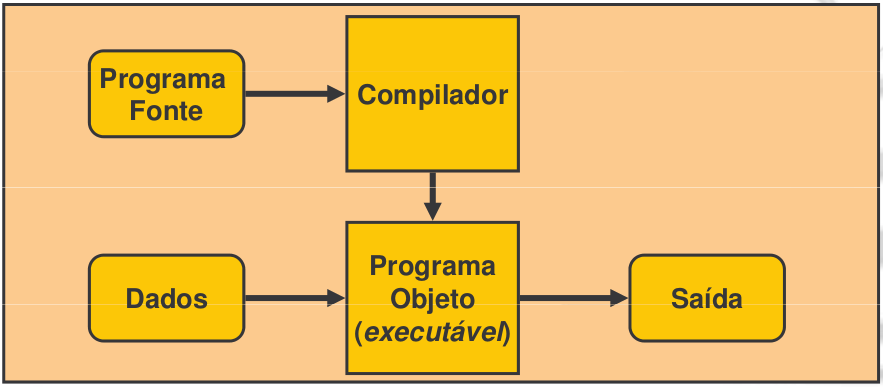
\includegraphics[height=0.4\paperheight]{fig/aula1/compilacao.png} \\
 \end{center} 
\end{frame}}
%----------------------------------------------------------------------------
\mode<presentation>{
\begin{frame}{Compilação}
\begin{itemize}
 \item O código fonte é compilado para uma plataforma e sistema operacional específico.
\end{itemize}
\begin{center}
   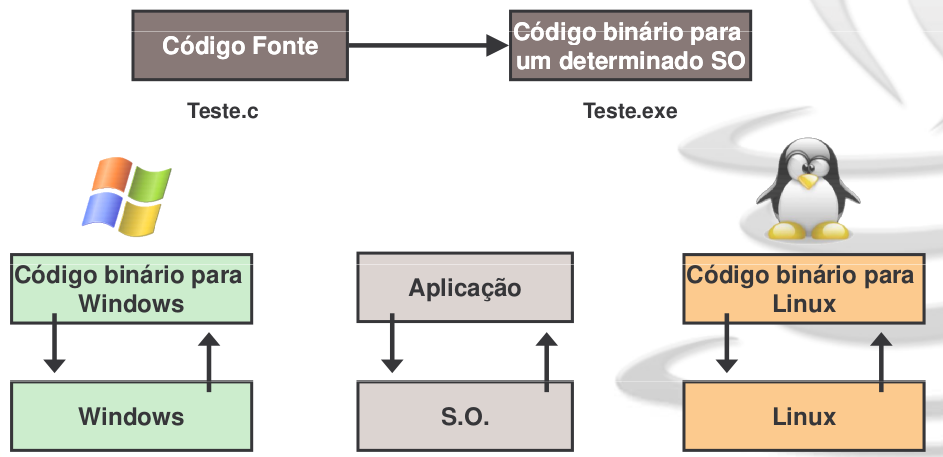
\includegraphics[height=0.5\paperheight]{fig/aula1/compilacao_2.png} \\
 \end{center} 
\end{frame}}
%----------------------------------------------------------------------------
\mode<presentation>{
\begin{frame}{Interpretação}
\begin{itemize}
 \item Examina o programa fonte, e executa cada instrução;
  \item A Interpretação é feita instrução a instrução;
\end{itemize}
\begin{center}
   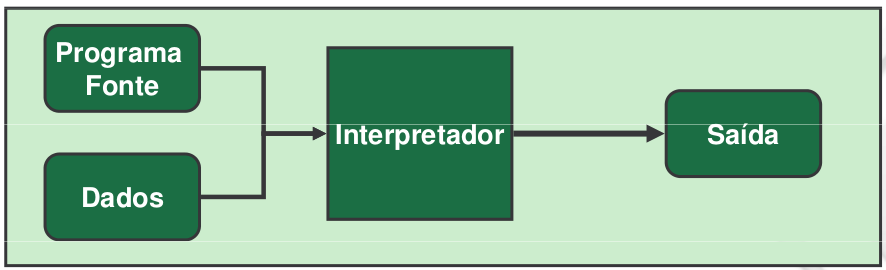
\includegraphics[height=0.3\paperheight]{fig/aula1/interpretacao.png} \\
 \end{center} 
\end{frame}}
%----------------------------------------------------------------------------
\mode<presentation>{ 
\begin{frame}{Compilação vs Interpretação}
\begin{center}
   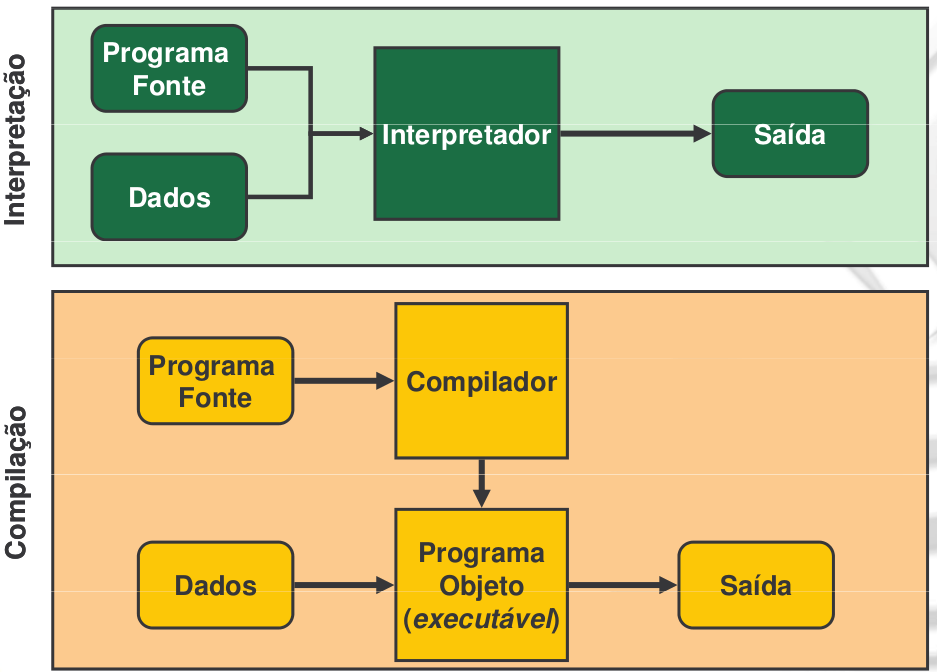
\includegraphics[height=0.65\paperheight]{fig/aula1/comp_vs_interp.png} \\
 \end{center} 
\end{frame}}
%----------------------------------------------------------------
\section{Atividade I}
\mode<presentation>{ \begin{frame}{Malhação cerebral}
 \vspace{2cm}
 \begin{enumerate}
 	 \item  Escreva com suas palavras o processo de compilação e interpretação. 
 	 \item Escreva quais as vantagens e desvantagens de cada método.

 \end{enumerate}

\end{frame}}
%----------------------------------------------------------------
\section{História da linguagem Java}
\mode<presentation>{ \begin{frame}{Java, como começou...}
 \begin{itemize}
  \item No ano de 1991 a Sun financiou um projeto de pesquisa interno de codinome Green, 
 chefiado por James Gosling e que criou uma linguagem baseada em C e C++ chamada Oak 
 (carvalho) para dispositivos eletrônicos inteligentes.
   \item Como o projeto não alcançou os resultados de mercado esperados, e em 1993 
 a World Wide Web explodiu em popularidade nos EUA, a Sun resolveu adaptar o projeto para 
 ser usado no desenvolvimento de conteúdo dinâmico para Web.
\end{itemize}
\end{frame}}
%----------------------------------------------------------------
\mode<presentation>{ \begin{frame}{Java, como começou...}
\begin{columns}
 \begin{column}{0.6\textwidth}
  \begin{itemize}
    \item Como já existia uma linguagem chamada Oak o nome foi trocado por Java (em 
 homenagem a um tipo de café importado que a equipe tomava numa cafeteria perto da empresa);
     \item Em 23 de maio de 1995 a Sun apresentou oficialmente a linguagem Java ao mercado, 
 na conferência SunWorld. E o seu mascote duke.
  \end{itemize}
 \end{column}

 \begin{column}{0.3\textwidth}
  \begin{center}
   
\includegraphics[height=0.5\paperheight]{fig/aula1/duke.png} \\
 \end{center}
 \end{column}
\end{columns}
 
\end{frame}}
%----------------------------------------------------------------
\section{Java}
\mode<presentation>{ \begin{frame}{Como java funciona?} 
  \begin{center}
   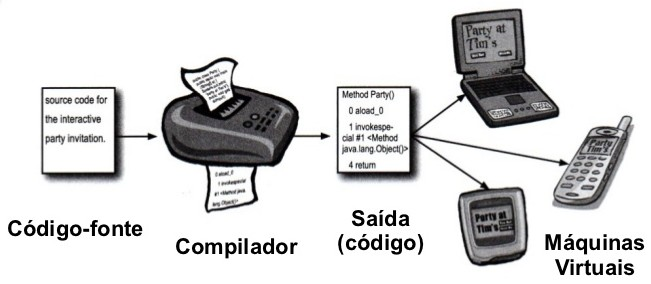
\includegraphics[height=0.5\paperheight]{fig/aula1/funcionamento_java.jpg} \\
 \end{center}

\end{frame}}
%----------------------------------------------------------------
\mode<presentation>{ \begin{frame}{Fases de um programa Java} 
  \begin{center}
   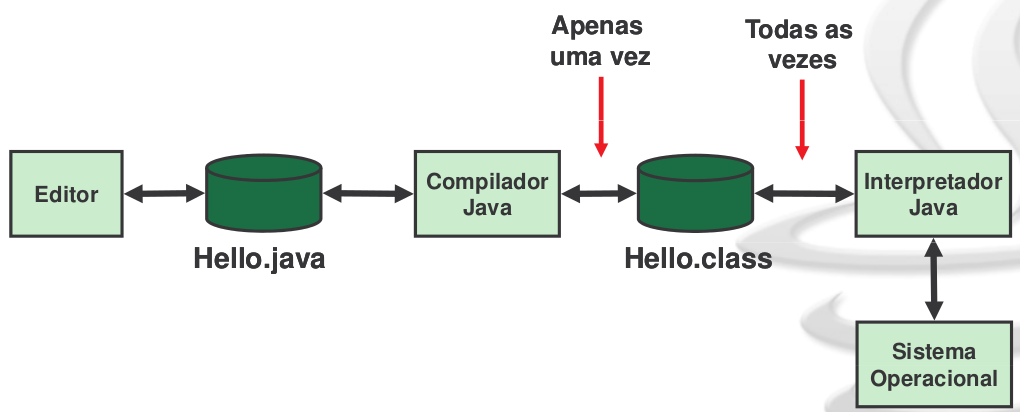
\includegraphics[height=0.5\paperheight]{fig/aula1/fases_java.png} \\
 \end{center}

\end{frame}}
%----------------------------------------------------------------
\section{Máquina Virtual Java}
\mode<presentation>{ \begin{frame}{Máquina Virtual} 
A arquitetua da Linguagem Java se baseia na existência de uma máquina virtual (JVM) que deixa 
transparente para a aplicação a existência do Sistema Operacional e do Hardware.
  \begin{center}
   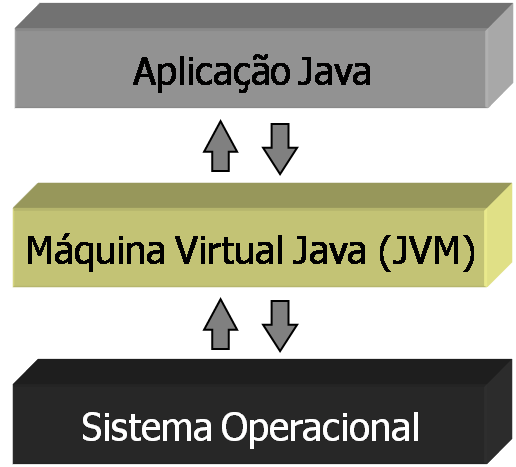
\includegraphics[height=0.5\paperheight]{fig/aula1/jvm-01.png} \\
 \end{center}

\end{frame}}
%----------------------------------------------------------------------
\mode<presentation>{ \begin{frame}{Máquina Virtual} 
A arquitetua da Linguagem Java se baseia na existência de uma máquina virtual (JVM) que deixa 
transparente para a aplicação a existência do Sistema Operacional e do Hardware.\\

\textcolor{red}{Qual a vantagem disso??}
  
  \begin{center}
   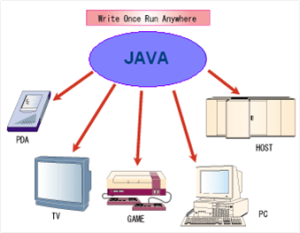
\includegraphics[height=0.45\paperheight]{fig/aula1/jvm-02.png} \\
 \end{center}

\end{frame}}

%----------------------------------------------------------------------
\mode<presentation>{ \begin{frame}{Máquina Virtual} 
``Máquina Virtual'' que roda as aplicações Java:
\begin{itemize}
 \item Funciona como um interpretador;
  \item Checagem de erros em tempo de execução;
  \item Garbage Collector (GC) - Coletor de lixo;
  \item Torna a linguagem independendente de plataformas (Windows, Linux, MacOS, ...);
  \item ``Write once. Run anywhere''.
\end{itemize}
\end{frame}}
%----------------------------------------------------------------------
\section{Plataforma}
\mode<presentation>{ \begin{frame}{Tecnologia Java} 
  \begin{center}
   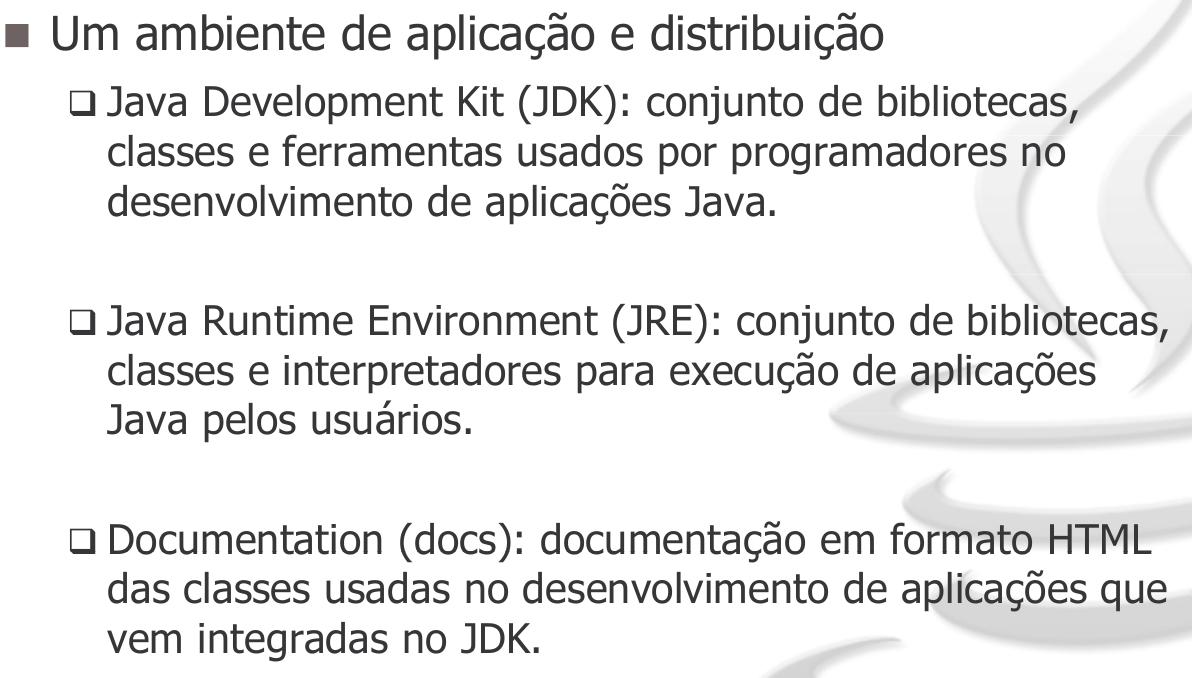
\includegraphics[height=0.6\paperheight]{fig/aula1/plataforma.png} \\
 \end{center}

\end{frame}}
%----------------------------------------------------------------------
\mode<presentation>{ \begin{frame}{Tecnologia Java} 
  \begin{center}
   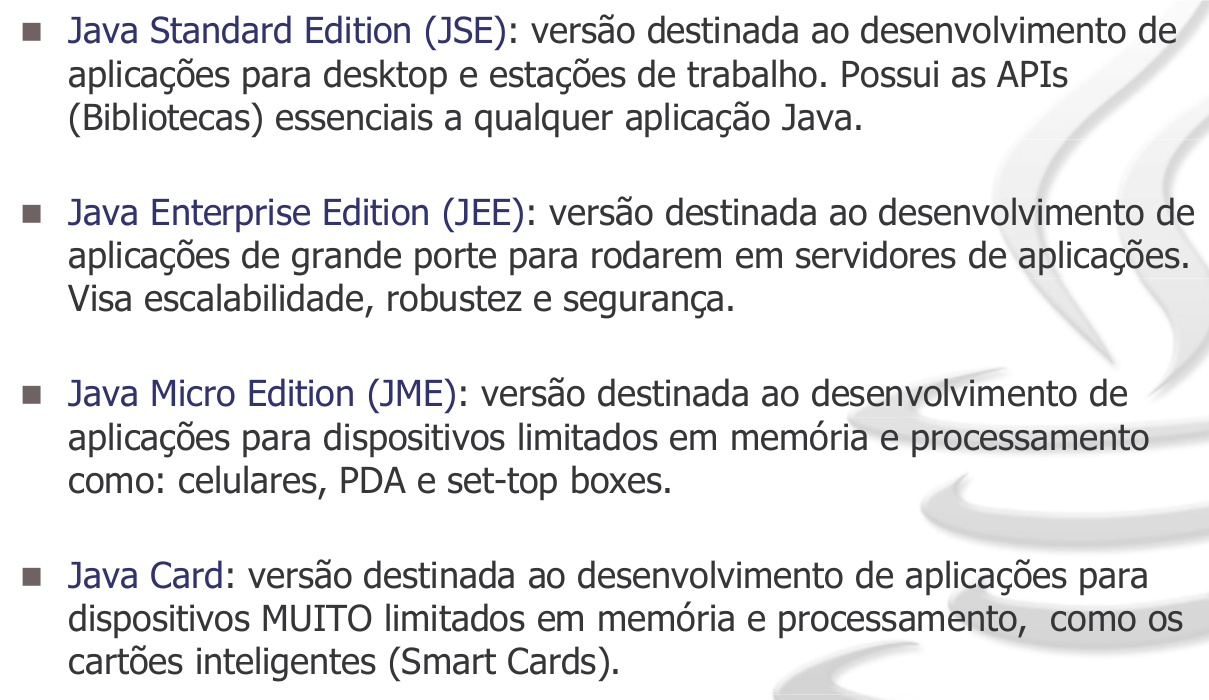
\includegraphics[height=0.6\paperheight]{fig/aula1/plataformas.png} \\
 \end{center}

\end{frame}}
%----------------------------------------------------------------------
\section{Arquivos}
\mode<presentation>{ \begin{frame}{Arquivos Java} 
  \begin{center}
   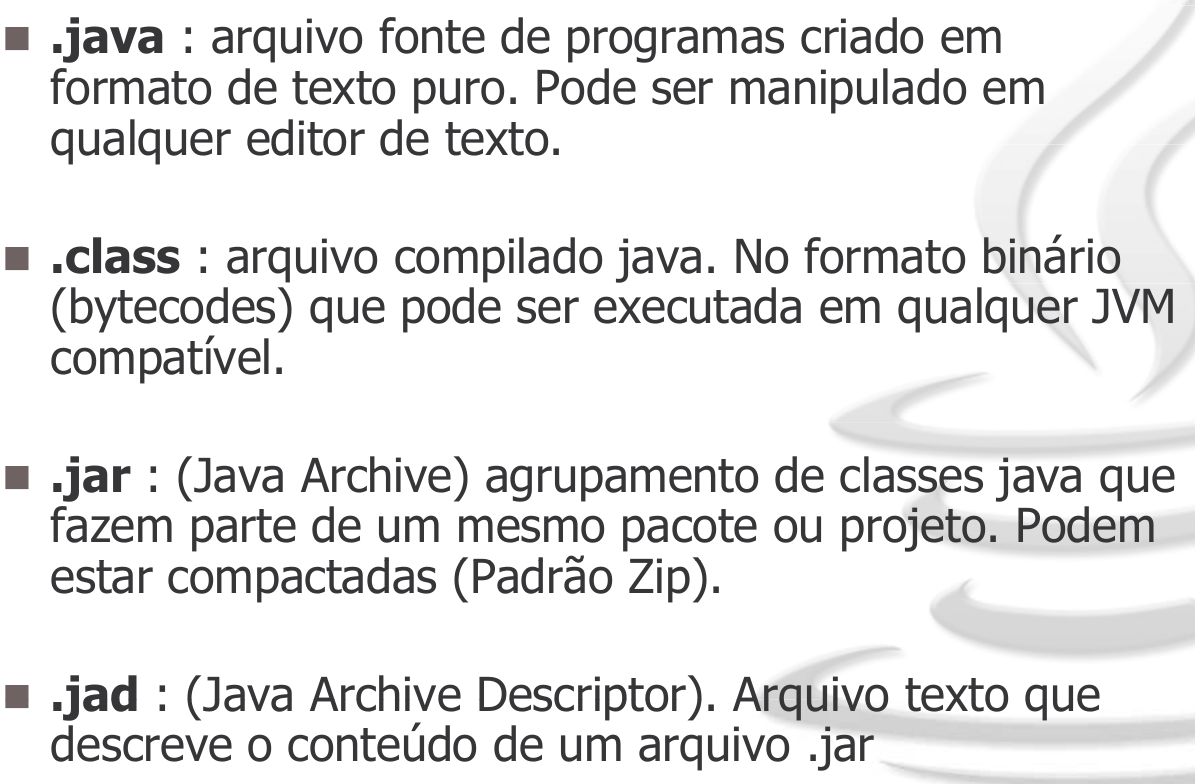
\includegraphics[height=0.65\paperheight]{fig/aula1/arquivos.png} \\
 \end{center}

\end{frame}}
%----------------------------------------------------------------------
\section{Atividades II}
\mode<presentation>{ \begin{frame}{Malhação Cerebral}
 \begin{enumerate}
  \item Descreva com detalhes as fases do desenvolvimento de um programa em JAVA.
   \item Escreva sobre a máquina virtual.
 \end{enumerate}
 \end{frame}}
%----------------------------------------------------------------------
\mode<presentation>{ \begin{frame}{O que cada linha de código faz?} 
  \begin{center}
   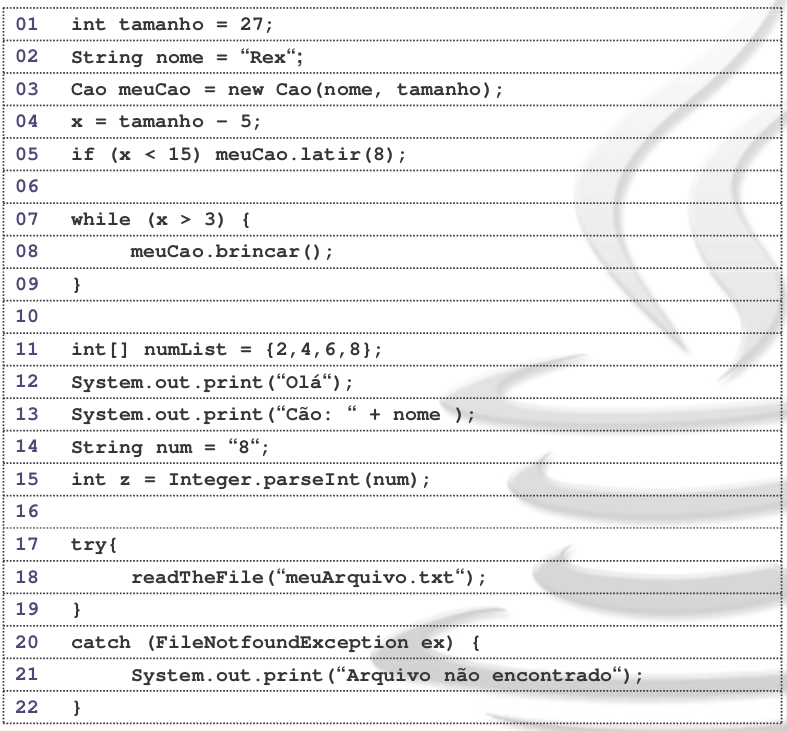
\includegraphics[height=0.7\paperheight]{fig/aula1/codigo_ativ2.png} \\
 \end{center}

\end{frame}}
%----------------------------------------------------------------------
\mode<presentation>{ \begin{frame}{O que cada linha de código faz?} 
  \begin{center}
   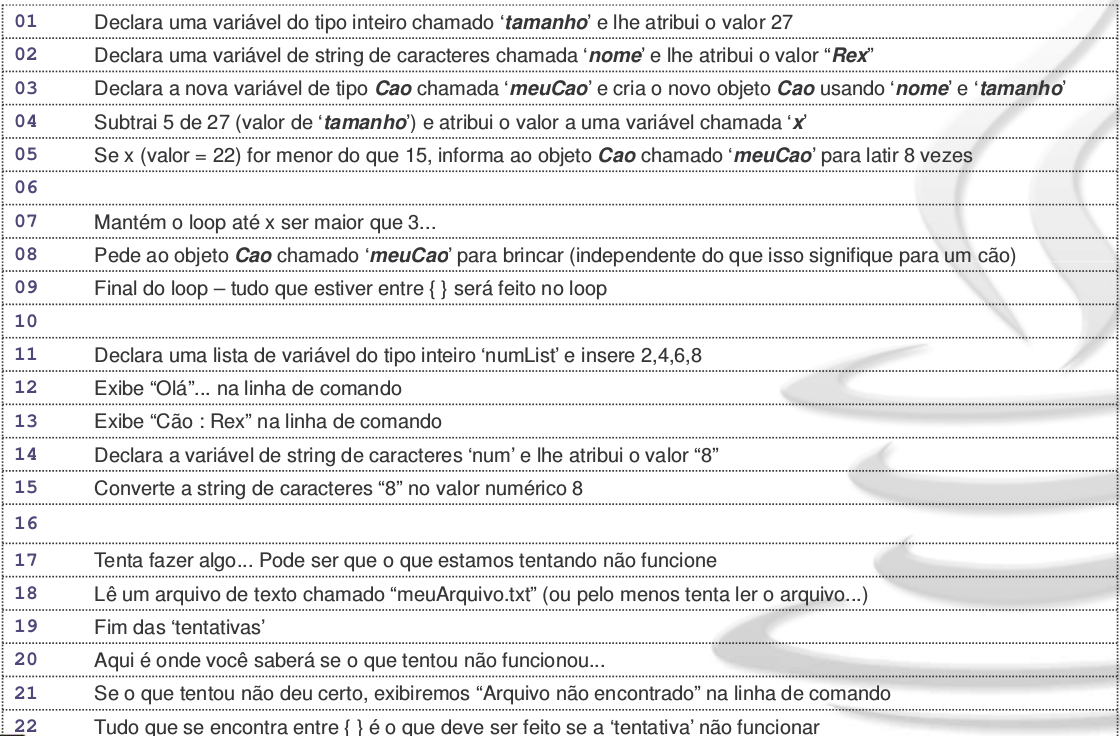
\includegraphics[height=0.7\paperheight]{fig/aula1/codigo_resp_ativ2.png} \\
 \end{center}

\end{frame}}
\section{O programa}
\mode<presentation>{ \begin{frame}{O programa JAVA}
\begin{itemize}
 \item Em Java tudo fica em uma classe;
  \item Geralmente cada classe fica em um arquivo (padrão de 
 desenvolvimento);
  \item O arquivo deve ter o mesmo nome da classe com a extensão .java;
  \item Ao executar um programa, você estará executando uma classe;
  \item Java é \textit{sensitive case}: \textbf{Java != java}
\end{itemize}
\end{frame}}
%----------------------------------------------------------------------------
\mode<presentation>{ \begin{frame}{Definições}
  \begin{columns}
  \begin{column}{0.8\textwidth} 
  \begin{itemize}
  \item Console
  \begin{itemize}
   \item Onde se executa os comandos do SO. \textbf{Exemplo:} Prompt de 
comandos (Windows)
  \end{itemize}
   \item Editor de texto
    \begin{itemize}
      \item \textbf{Exemplo:} Notepad (Windows)
    \end{itemize}
   \item Ambiente de Desenvolvimento Integrado (IDE): É um aplicativo
 que provê: um editor de códigos, um compilador e/ou interpretador, depurador.
    \begin{itemize}
      \item \textbf{Exemplo:} NetBeans, Eclipse
      \end{itemize}
    \end{itemize}
  \end{column}
  \begin{column}{0.2\textwidth}
   \begin{center}
    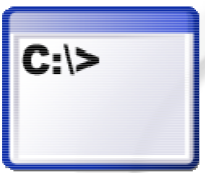
\includegraphics[height=0.1\paperheight]{fig/aula1/prompt.png} \\
    \vspace{0.5cm}
    
\includegraphics[height=0.1\paperheight]{fig/aula1/editor.png} \\
    \vspace{0.5cm}
    
\includegraphics[height=0.3\paperheight]{fig/aula1/ide.png} \\
   \end{center} 
  \end{column}
 \end{columns}

\end{frame}}
%----------------------------------------------------------------------------
\section{Hello World}
\mode<presentation>{ \begin{frame}{Primeiro programa em Java}
\begin{enumerate}
 \item Iniciar o editor de texto;
  \item Escrever o código utilizando o editor;
  \item Salvar o código com o nome \textcolor{blue}{cod/Ola.java}
  \item Abrir o console
  \item Entrar na pasta onde o arquivo de código fonte
 (.java) esta salvo
  \item Compilar o código fonte: \textcolor{red}{javac Ola.java}
  \item Executar o programa: \textcolor{red}{java Ola}
\end{enumerate}
\end{frame}}
%----------------------------------------------------------------------------
\mode<presentation>{ \begin{frame}{Primeiro programa Java}
\begin{center}
    \lstinputlisting[language=Java, linerange=1-5]{cod/Ola.java}
    %\lstinputlisting[linerange={1-5}]{./codigo/Ola.java}
  \end{center}
  
  \begin{itemize}
   \item cd C:$<caminho-pasta>$
   \item javac Ola.java
   \item java Ola
  \end{itemize}

\end{frame}}
%----------------------------------------------------------------------------
\section{Método main()}
\mode<presentation>{ \begin{frame}{O método main()}
  \begin{itemize}
   \item O método main() é onde a execução inicia
    \item Executar um programa, é o mesmo que dizer a Máquina Virtual
   (JVM) para carregar a classe e executar o método main()
    \item O método main() sempre é chamado de forma automática
    \item Nem toda classe exige um método main()
    \item Não importa quantas classes seu programa possui
   \item Mas deverá possuir apenas um método main() - desse modo o programa 
   torna-se ``executável''
  \end{itemize}

\end{frame}}
%----------------------------------------------------------------
\mode<presentation>{ \begin{frame}{O método main()}
  Exemplos:
  
  \begin{itemize}
   \item O parâmetro do método main é um vetor formado por textos 
   passados via linha de comando
    \item O parâmetro pode ser declarado de formas diferentes, seu 
   \textbf{nome} \textcolor{red}{não importa}, porém, obrigatóriamente 
   deve ser um array de String
  \end{itemize}
\end{frame}}
%----------------------------------------------------------------
\mode<presentation>{ \begin{frame}{O método main()}
  \begin{center}
    \lstinputlisting[linerange={1-5}]{./cod/Main.java}
  \end{center}
  \begin{itemize}
   \item Qualquer distorção neste cabeçalho, a JVM não identificará o método
   e ocorrerá um erro durante a execução da classe.
  \end{itemize}
\end{frame}}
%----------------------------------------------------------------
\section{Saída de dados padrão}
\mode<presentation>{ \begin{frame}{Saída de dados}
 \begin{itemize}
  \item System.out...
   \item O método \textbf{\textcolor{red}{print}} imprime um conjunto 
  de dados e posiciona o cursor no final deles
   \item O método \textbf{\textcolor{red}{println}} imprime um conjunto de dados e posiciona o 
  cursor na próxima linha
   \item \textbf{\textcolor{red}{Ambos são métodos sobrecarregados}}, 
  ou seja, existem várias versões destes métodos (funcionam para diferentes 
  tipos e quantidades de parâmetros)
\end{itemize}
\end{frame}}
%----------------------------------------------------------------
\mode<presentation>{ \begin{frame}{Saída padrão (print e println)}
  \begin{center}
   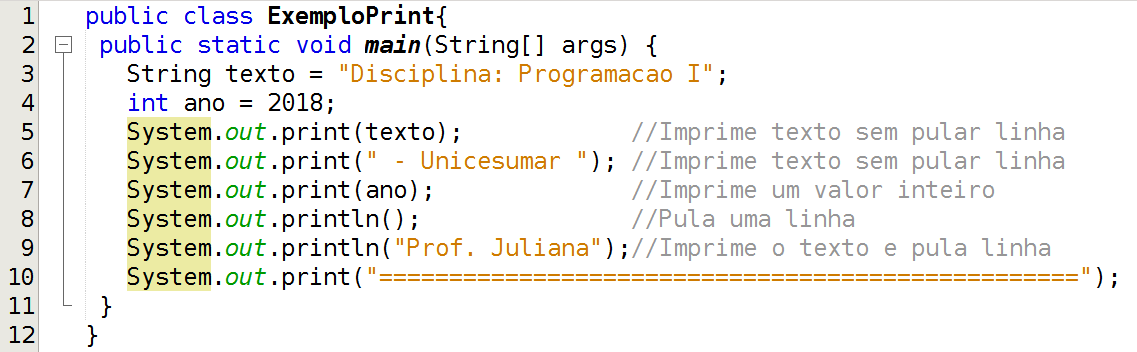
\includegraphics[height=0.4\paperheight]{fig/aula1/exemploPrint.png} \\
   
   \textbf{Saída}\\
   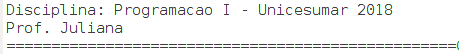
\includegraphics[height=0.1\paperheight]{fig/aula1/exemploPrintOut.png} \\
 \end{center}
\end{frame}}
%----------------------------------------------------------------
\mode<presentation>{ \begin{frame}{Exemplo 2 (print e println)}
  \begin{center}
    \lstinputlisting[linerange={1-7}]{./cod/ExemploPrint2.java}
   
   \textbf{Saída}\\
   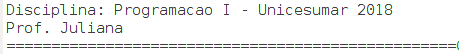
\includegraphics[height=0.1\paperheight]{fig/aula1/exemploPrintOut.png} \\
 \end{center}
\end{frame}}
%----------------------------------------------------------------------
\mode<presentation>{ \begin{frame}{print e println} 
\begin{itemize}
 \item Conseguimos a mesma saída;
  \item Com uma menor quantidade de comandos \textbf{print} e \textbf{println};
  \item Isso foi possível por causa so uso de dois operadores;
  \item Operador de concatenação ``+'';
  \item Operador de escape ``$\setminus n$''.
\end{itemize}
\end{frame}}

%-----------------------------------------------------------------------
\section{Leitura recomendada}
\mode<presentation>{ \begin{frame}{Leitura complementar}
 Para mais informações sobre JAVA, leia:\\
	\begin{columns}
	\begin{column}{0.5\textwidth}
	 Capítulo 1:
	 \cite{deitel2017java}
	\end{column}
	\begin{column}{0.4\textwidth}
	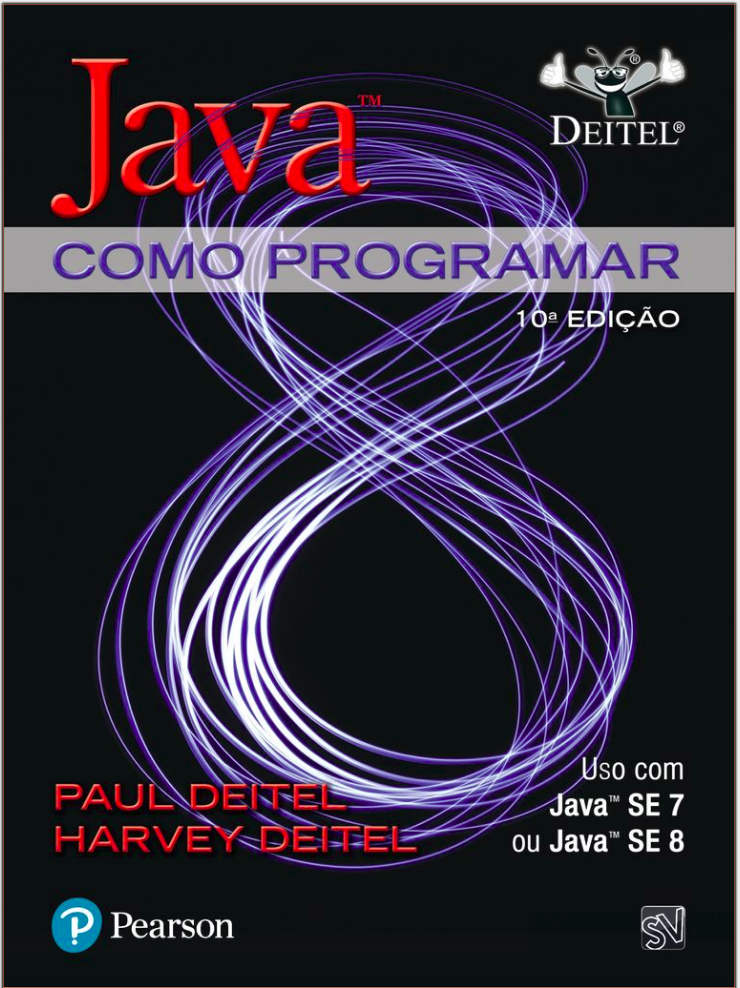
\includegraphics[height=0.6\paperheight]{fig/aula1/deitel2017java.png} 
	\end{column}
	\end{columns}
	\textcolor{red}{DISPONÍVEL NA BIBLIOTECA VIRTUAL}
\end{frame}}

 %----------------------------------------------------------------------------
 
 \mode<presentation>{ \begin{frame}{Referências}%[allowframebreaks]
 \small
 \begin{center}
 	\bibliographystyle{apalike}
	 \bibliography{ref_aula_progI}
 \end{center}
 \end{frame}}

\begin{figure}[!ht] \fbox{\includeslide[width=\textwidth]{slide:z}} \end{figure}
Text for notes goes here. 
\begin{itemize}
  \item List 1. 
  \item List 2. 
\end{itemize}


%%%%%%%%%%%%%%%%%% END MATTER %%%%%%%%%%%%%%%%%%
\end{document}